\RequirePackage{plautopatch}
\documentclass[english, dvipdfmx, a4paper]{jsarticle}
\usepackage[utf8]{inputenc}
\usepackage[top=10truemm, bottom=20truemm, left=15truemm, right=15truemm]{geometry} % mergin
\renewcommand{\headfont}{\bfseries}

% graphics
\usepackage{graphicx}
\usepackage{here}

% link

\usepackage{url}
\usepackage[dvipdfmx, linktocpage]{hyperref} 
\usepackage{xcolor}
\usepackage{pxjahyper}
\hypersetup{
	colorlinks=true,
	citecolor=blue,
	linkcolor=teal,
	urlcolor=orange,
}

% math

\usepackage{amsmath, amssymb} 
\usepackage{physics}
\usepackage{mathrsfs}
\usepackage{mathtools}
\usepackage{tensor}
\usepackage{simpler-wick}
% theoremstyle
\usepackage{amsthm}
\newtheoremstyle{break}
{\topsep}{\topsep}%
{}{}%
{\bfseries}{}%
{\newline}{}%
\theoremstyle{break}
\newtheorem{thm}{Theorem}[section]
\newtheorem{defn}[thm]{Definition}
\newtheorem{eg}[thm]{Example}
\newtheorem{cl}[thm]{Claim}
\newtheorem{cor}[thm]{Corollary}
\newtheorem{fact}[thm]{Fact}
\newtheorem{rem}[thm]{Remark}
\newtheorem{prob}{Problem}[section]

\makeatletter
\newenvironment{pr}[1][\proofnam]{\par
\topsep6\p@\@plus6\p@ \trivlist
\item[\hskip\labelsep{\itshape #1}\@addpunct{\bfseries}]\ignorespaces
}{%
\endtrivlist
}
\newcommand{\proofnam}{\underline{Derivation.}}
\makeatother

% ordinary
\newcommand{\R}{\mathbb{R}}
\newcommand{\C}{\mathbb{C}}
\newcommand{\Z}{\mathbb{Z}}
	
\newcommand{\e}{\mathrm{e}}
\renewcommand{\i}{\mathrm{i}}
% Physics %%%%%%%%%%%%%%%%%%%%%%%%%%%%%%%%%%%%
	
% Feynman slash
\newcommand{\slashed}[1]{#1\!\!\!/}

% time ordering

\newcommand{\T}{\mathcal{T}}
\newcommand{\M}{\mathcal{M}}
\renewcommand{\P}{\mathcal{P}}
\usepackage[compat=1.1.0]{tikz-feynhand}

\newcommand{\elec}{\mathsf{e}}
\newcommand{\muon}{\mathrm{\mu}}
% order

%Lie algebra
\renewcommand{\O}{\mathcal{O}}
\newcommand{\SO}{\mathrm{SO}}
\newcommand{\so}{\mathfrak{so}}
\newcommand{\SU}{\mathrm{SU}}
\newcommand{\su}{\mathfrak{su}}
\newcommand{\SP}{\mathrm{SP}}
\renewcommand{\sp}{\mathfrak{sp}}
\newcommand{\SL}{\mathrm{SL}}
\renewcommand{\sl}{\mathfrak{sl}}
\newcommand{\GL}{\mathrm{GL}}
\newcommand{\gl}{\mathfrak{gl}}
\newcommand{\U}{\mathrm{U}}
\renewcommand{\u}{\mathfrak{u}}


% number

\makeatletter
\@addtoreset{equation}{section}
\makeatother
\numberwithin{equation}{section}
\renewcommand{\thefootnote}{\roman{footnote}.}
\renewcommand{\appendixname}{Appendix }
\newcommand{\textref}[1]{(PS. #1)}
\newcommand{\intp}[2][3]{\int \frac{\dd[#1]{#2}}{(2\pi)^{#1}}}
\title{場の理論ゼミ}
\author{Toshiya Tanaka}
\date{\today}
\begin{document}
	\maketitle
	\section*{はじめに}
	\begin{itemize}
		\item M1の前期の授業でPeskin--Schr\"{o}derの場の理論の本\cite{Peskin1995}を読むことになったので,学びを記録しようと思います.
		\item 教科書中の式は\textref{式番号}のように記します.
		\item 教科書の公式ページは\href{https://physics.weber.edu/schroeder/qftbook.html}{こちら}です.
		\item 5章までは富山大学理論物理学研究室でやったゼミのまとめが\href{https://toshitnk.github.io/hp/seminars/Peskin.html}{こちら}にあります.
	\end{itemize}

	\setcounter{section}{5}
	\section{Radiative correction}
\begin{itemize}
	 \item bremsstrahlungで出てくるphotonは低エネルギー過ぎて観測できないので,実験上は
	 \begin{center}
	 	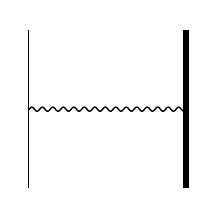
\begin{tikzpicture}
			\begin{feynhand}
				\vertex (a) at (-1, -1);
				\vertex (b) at (-1, 1);
				\vertex (c) at (1, -1);
				\vertex (d) at (1, 1);
				\propag[plain, line width=2pt] (c) to (d);
				\propag[plain] (a) to (b);

				\vertex (e) at (-1, 0);
				\vertex (f) at (1, 0);
				\propag[photon] (e) to (f);
			\end{feynhand}
		\end{tikzpicture}
		\qquad{}と\qquad{}
	 	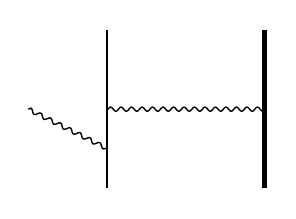
\begin{tikzpicture}
			\begin{feynhand}
				\vertex (a) at (-1, -1);
				\vertex (b) at (-1, 1);
				\vertex (c) at (1, -1);
				\vertex (d) at (1, 1);
				\propag[plain, line width=2pt] (c) to (d);
				\propag[plain] (a) to (b);

				\vertex (e) at (-1, 0);
				\vertex (f) at (1, 0);
				\propag[photon] (e) to (f);

				\vertex (h) at (-1, -0.5);
				\vertex (g) at (-2, 0);
				\propag[photon] (h) to (g);
			\end{feynhand}
		\end{tikzpicture}
	\end{center}
	は区別できないのだが,計算上はすべてのprocessを取り込む必要がある.
	masslessの粒子がいると,このようにいくらで低エネルギーのものをとりこんで,
	エネルギースペクトラムは$m_\elec$から上は連続的になる.

	\item \textref{6.1}以外にheavy particleを含むloop diagramが次の6種類ある.
	loop diagramとは,外線の運動量を決めても内線の運動量がuniqueに決まらないdiagramであることに注意.
	\begin{center}
		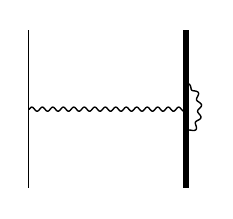
\begin{tikzpicture}
			\begin{feynhand}
				\vertex (a) at (-1, -1);
				\vertex (b) at (-1, 1);
				\vertex (c) at (1, -1);
				\vertex (d) at (1, 1);
				\propag[plain, line width=2pt] (c) to (d);
				\propag[plain] (a) to (b);

				\vertex (e) at (-1, 0);
				\vertex (f) at (1, 0);
				\propag[photon] (e) to (f);

				\vertex (h) at (1, -0.3);
				\vertex (g) at (1, 0.3);
				\propag[photon] (h) to  [out=0, in=0](g);
			\end{feynhand}
		\end{tikzpicture}
		,\quad
		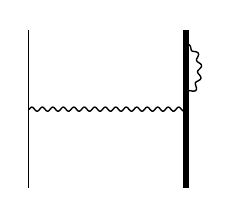
\begin{tikzpicture}
			\begin{feynhand}
				\vertex (a) at (-1, -1);
				\vertex (b) at (-1, 1);
				\vertex (c) at (1, -1);
				\vertex (d) at (1, 1);
				\propag[plain, line width=2pt] (c) to (d);
				\propag[plain] (a) to (b);

				\vertex (e) at (-1, 0);
				\vertex (f) at (1, 0);
				\propag[photon] (e) to (f);

				\vertex (h) at (1, 0.2);
				\vertex (g) at (1, 0.8);
				\propag[photon] (h) to [out=0, in=0](g);
			\end{feynhand}
		\end{tikzpicture}
		,\quad
		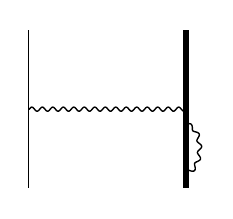
\begin{tikzpicture}
			\begin{feynhand}
				\vertex (a) at (-1, -1);
				\vertex (b) at (-1, 1);
				\vertex (c) at (1, -1);
				\vertex (d) at (1, 1);
				\propag[plain, line width=2pt] (c) to (d);
				\propag[plain] (a) to (b);

				\vertex (e) at (-1, 0);
				\vertex (f) at (1, 0);
				\propag[photon] (e) to (f);

				\vertex (h) at (1, -0.2);
				\vertex (g) at (1, -0.8);
				\propag[photon] (h) to [out=0, in=0] (g);
			\end{feynhand}
		\end{tikzpicture}
		, \quad
		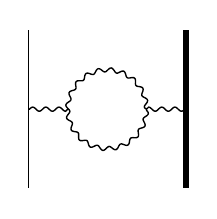
\begin{tikzpicture}
			\begin{feynhand}
				\vertex (a) at (-1, -1);
				\vertex (b) at (-1, 1);
				\vertex (c) at (1, -1);
				\vertex (d) at (1, 1);
				\propag[plain, line width=2pt] (c) to (d);
				\propag[plain] (a) to (b);

				\vertex (e) at (-1, 0);
				\vertex (f) at (-0.5, 0);
				\propag[photon] (e) to (f);

				\vertex (g) at (1, 0);
				\vertex (h) at (0.5, 0);
				\propag[photon] (g) to (h);
				\vertex (i) at (0, 0.5);
				\vertex (j) at (0, -0.5);
				\propag[photon] (h) to [out=270, in=0] (j) to [out=180, in=270] (f) to [out=90, in=180] (i) to [out=0, in=90] (h);
			\end{feynhand}
		\end{tikzpicture}
		,\quad
		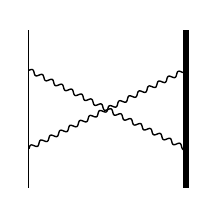
\begin{tikzpicture}
			\begin{feynhand}
				\vertex (a) at (-1, -1);
				\vertex (b) at (-1, 1);
				\vertex (c) at (1, -1);
				\vertex (d) at (1, 1);
				\propag[plain, line width=2pt] (c) to (d);
				\propag[plain] (a) to (b);

				\vertex (e) at (1, 0.5);
				\vertex (f) at (1, -0.5);
				\vertex (g) at (-1, 0.5);
				\vertex (h) at (-1, -0.5);

				\propag[photon] (g) to (f);
				\propag[photon] (h) to (e);
			\end{feynhand}
		\end{tikzpicture}
		, \quad
		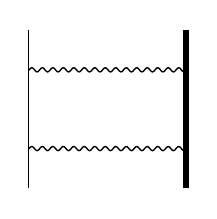
\begin{tikzpicture}
			\begin{feynhand}
				\vertex (a) at (-1, -1);
				\vertex (b) at (-1, 1);
				\vertex (c) at (1, -1);
				\vertex (d) at (1, 1);
				\propag[plain, line width=2pt] (c) to (d);
				\propag[plain] (a) to (b);

				\vertex (e) at (1, 0.5);
				\vertex (f) at (1, -0.5);
				\vertex (g) at (-1, 0.5);
				\vertex (h) at (-1, -0.5);

				\propag[photon] (g) to (e);
				\propag[photon] (h) to (f);
			\end{feynhand}
		\end{tikzpicture}
	\end{center}
	\item \textref{Fig. 7.2}などはmassless photonがいないと仮定して,スペクトラムを書いている.
	このときは図にあるように$2m_\elec$から状態が連続的に分布する.
	状態があると,相関関数のFourier変換がpoleを持つらしく,連続spectrumだと大体poleが連続的に分布すると思えば,そこにbranch cutが走ることになる.
	\end{itemize}




	\begin{itemize}
	\item \textref{6.4}では$m\epsilon$を改めて$\epsilon$とおいている.

	\item \textref{6.5}の計算で$1/k^2$のpoleを両方下に下げる遅延条件を設定することは,今$t=0$で瞬間的に加速されることを考えているので,それ以前に放射の場はなくて,その後には存在するという境界条件を課していることと思える
	\footnote{今,微分方程式をFourier変換したものを考えており,このようなpoleをずらす操作は適切な境界条件を与えていると思える.}.

	$t>0$の場合でも放射が起こるのか,と混乱したが,そうではなくて$t=0$の瞬間に放射が起こったものが$t>0$でも残っていると思うと教えてもらった.
	\item \textref{6.5}の$k^0$についての積分を行う際に,複素関数として,上(下)半平面に積分路を追加してそれがゼロに飛ぶことを使うが,
	$\e^{\i kz} = \e^{\i kR\cos\theta - kR\sin\theta}$をゼロに飛ばしたときに$\theta \sim 0$の範囲で本当に収束するのかという質問がでた.
	これは,一般論としては\href{https://ja.wikipedia.org/wiki/\%E3\%82\%B8\%E3\%83\%A7\%E3\%83\%AB\%E3\%83\%80\%E3\%83\%B3\%E3\%81\%AE\%E8\%A3\%9C\%E9\%A1\%8C}{Jordanの補題}というのがあって,その証明を追えばよいのだが,収束することは次のように言える.

	まず,積分について$f(z)$を$M/R^k$, $(k>0)$程度で抑えられる関数\footnote{たとえば$1/(k^2 + m^2)$なら$k=3$くらい,今の場合の$1/(k^4(k+m)(k-m))$だと$k=5$など.}として,
	\begin{align}
		\int \dd{z}f(z)e^{\i kz} &= \int_{0}^{\pi} \dd{\theta}\i R\e^{\i\theta} f(R\e^{\i\theta})\e^{\i kR\cos\theta - kR\sin\theta}\\
		&= 2\int_{0}^{\pi/2} \dd{\theta}\i R\e^{\i\theta} f(R\e^{\i\theta})\e^{\i kR\cos\theta - kR\sin\theta}\\
	\end{align}
	とできる.$\pi/2 \leq \theta \leq \pi$については$\theta \to \pi-\theta$としてまとめた.

	$0 \leq \theta \leq \pi/2$においては$\sin\theta \geq 2\theta/\pi$
	が成り立つので,
	\begin{align}
		\abs{\int_{0}^{\pi/2} \dd{\theta}\i R\e^{\i\theta} f(R\e^{\i\theta})\e^{\i kR\cos\theta - kR\sin\theta}}
		&\leq \int_{0}^{\pi/2}\dd{\theta}R\abs{f(R\e^{\i\theta})}\e^{-kR\sin\theta}\\
		&\leq \frac{M}{R^k}\int_{0}^{\pi/2}\dd{\theta}\e^{-kR2\theta/\pi}\\
		&= \frac{M}{R^k}\frac{\pi}{2kR}(1 - \e^{-kR})\\
		&\leq \frac{\pi}{2kR^k}M \underset{R\to\infty}{\to} 0
	\end{align}
	となる.
	\item p.178の一番下の式からp.179の最初の式で負号が消えているのは,$p^{\mu} = (p^0, \vec{0})$と設定したので,$k^0 = \vec{k}\cdot \vec{p}/p^0 = 0$だから,分母の$k^2 = -\abs*{\vec{k}}^2$の負号が出てくるからである.

	\item \textref{6.10}の絶対値はベクトルの絶対値で,\textref{6.8}で実数に設定しているので複素共役をとる必要はない.
	また,$1/8$の係数は,エネルギーの定義の$1/2$と$\R\ni a = (z+z^*)/2$と書くときの$1/2$のfactor 2つ分によりついている.

	\item \textref{6.10}の$\vec{B}$側の評価で,形は$\vec{E}$のほうと同じだから,
	\begin{equation}
		\frac{1}{2}\int\dd[3]{x}\abs*{\vec{B}(x)}^2
		= \frac{1}{8}\intp[3]{k}
		\qty(\vec{\mathcal{B}}(\vec{k})\cdot \vec{\mathcal{B}}(\vec{-k})\e^{-2\i k^0t}
		+ 2\vec{\mathcal{B}}(\vec{k}) \cdot \vec{\mathcal{B}}^{*}(\vec{k})
		+ \vec{\mathcal{B}}^{*}(\vec{k}) \cdot \vec{\mathcal{B}}^{*}(\vec{-k})\e^{2\i k^0t})
	\end{equation} 
	となる.
	ここで,ベクトル解析の式$(\vec{A}\times\vec{B})\cdot(\vec{C}\times \vec{D}) = (\vec{A}\cdot \vec{C})(\vec{B}\cdot \vec{D}) - (\vec{A}\cdot\vec{D})(\vec{B}\cdot \vec{C})$をつかい,$\vec{\mathcal{B}} = \hat{\vec{k}} \times \vec{\mathcal{E}}$であることと$\vec{k} \cdot \vec{\mathcal{E}} = 0$を考慮すると$\vec{\mathcal{B}}(\vec{k})\cdot\vec{\mathcal{B}}(-\vec{k}) = -\vec{\mathcal{E}}(\vec{k})\cdot\vec{\mathcal{E}}(-\vec{k})$などとなり,$\e^{\pm \i k^0t}$の項は足すと消える.

	\item 偏光ベクトル$\epsilon^{\mu}$は四元ベクトルだが,ゲージ対称性で一成分,zero normのunphysical stateを消すために一成分消えるので,独立なものは二つ.
	\item \textref{6.13}で$\sum \epsilon_\mu\epsilon_\nu^{*}$を$-g_{\mu\nu}$に置き換えてよいのは,$k_{\mu}(p'^{\mu}/(k\cdot p') - p^{\mu}/(k\cdot p)) = 0$がなりたつ.
	\textref{5.79}あたりの議論を追うと
	まず,$k^{\mu*} = (k, 0,0, k)$, $\epsilon^1 = (0, 1, 0, 0)$, $\epsilon^2 = (0, 0, 1, 0)$をとり,
	$k_{\mu}f^{\mu} = 0 $が成り立っている.$k$の取り方から,
	$kf^0 - kf^3 = 0$がわかり,
	$\sum \epsilon_\mu\epsilon_\nu f^\mu f^{\nu *} = \abs{f^1}^2 L \abs{f^2}^2 = \abs{f^1}^2 + \abs{f^2}^2 + \abs{f^3}^2 - \abs{f^0}^2 = g_{\mu\nu}f^{\mu}f^{\nu * }$となるので,
	この置き換えをしてよいことがわかる.(逆に,この種の条件がない場合は置き換えができない.)
	

	\item p.181最後に積分の下端を設定するところの$\vec{v}$などはhigh energyを考えているので$\abs*{\vec{v}} \sim 1$であることに今後注意すべき.
	また,この下端の設定は任意性があり,今考えているのは放射が軸にほぼ平行な$\cos\theta \sim 1$あたりからの寄与がdominantであるからである.

	この設定に物理的解釈をつけようと思うと,後ろに放射することはないだろうとおもい,方向転換する角度でcutoffするという説明を教えてもらった.


	\item \textref{6.17}の$\approx 2\log(p\cdot p'/((E^2-\abs*{\vec{p}})/2))$への変形は,分母の$E^2(E-\abs*{\vec{p}}) \simeq (E+\abs*{\vec{p}})/2(E-\abs*{\vec{p}})$と考えるとよい.
	また,直接しらべるとこの途中式を経ず,最後の形にもっていくこともできるらしい. 
	\item \textref{6.17}の最後は等号だが近似を使っている.
\end{itemize}

	\bibliography{QFT}
	\bibliographystyle{ytamsalpha}
	%\bibliographystyle{ytamsbeta}
\end{document}
